\chapter{Two-source refractive index measurement}
\label{chap:refractive_index}

\section{Introduction}
\label{intro_ts}
In chapter \ref{chap:two_source}, the $0-\pi$ square-wave phase grating (SWPG) was introduced as a means of generating two intense duplicates of an input femtosecond mid-IR pulse.  An additional element of the SWPG is that it enables precise control over the relative phase between these two sources.  When used to generate high harmonics, this scheme enables the generation of two XUV sources whose relative phase is well controlled by the SWPG, and any small phase shift between the two harmonic beams is imprinted upon their interference pattern as a fringe shift in the far-field.  The idea is to now leverage this sensitivity to measure an induced phase shift between the two XUV sources.  In the experiment described in this chapter, the phase shift will be induced by introducing a thin condensed matter sample into only one of the two XUV sources.  Doing so enables us to extract both the real and imaginary part of the refractive index over a broad range of photon energies in the XUV.
\section{Complex refractive index}
The complex refractive index depends strongly on photon energy, and a cartoon of this is shown in figure \ref{fig:refractive_index_schematic}. We are interested in the refractive index in the XUV energy region, and in this energy region there are many resonances that correspond to transitions of core-level electrons to unoccupied states near the Fermi level (for the case of a condensed matter system)\cite{stohrNEXAFSSpectroscopy1992, attwoodSoftXraysExtreme2000}.  Complicated fine structure can emerge near these resonances that correspond to the local electronic and geometric environment\cite{stohrNEXAFSSpectroscopy1992, attwoodSoftXraysExtreme2000}.  Thus, the ability to measure both the real and imaginary parts of the complex refractive index can be important for many experiments using XUV light generated by HHG\cite{kaplanFemtosecondTrackingCarrier2018,  cirriAchievingSurfaceSensitivity2017}.

\begin{figure}
	\centering
	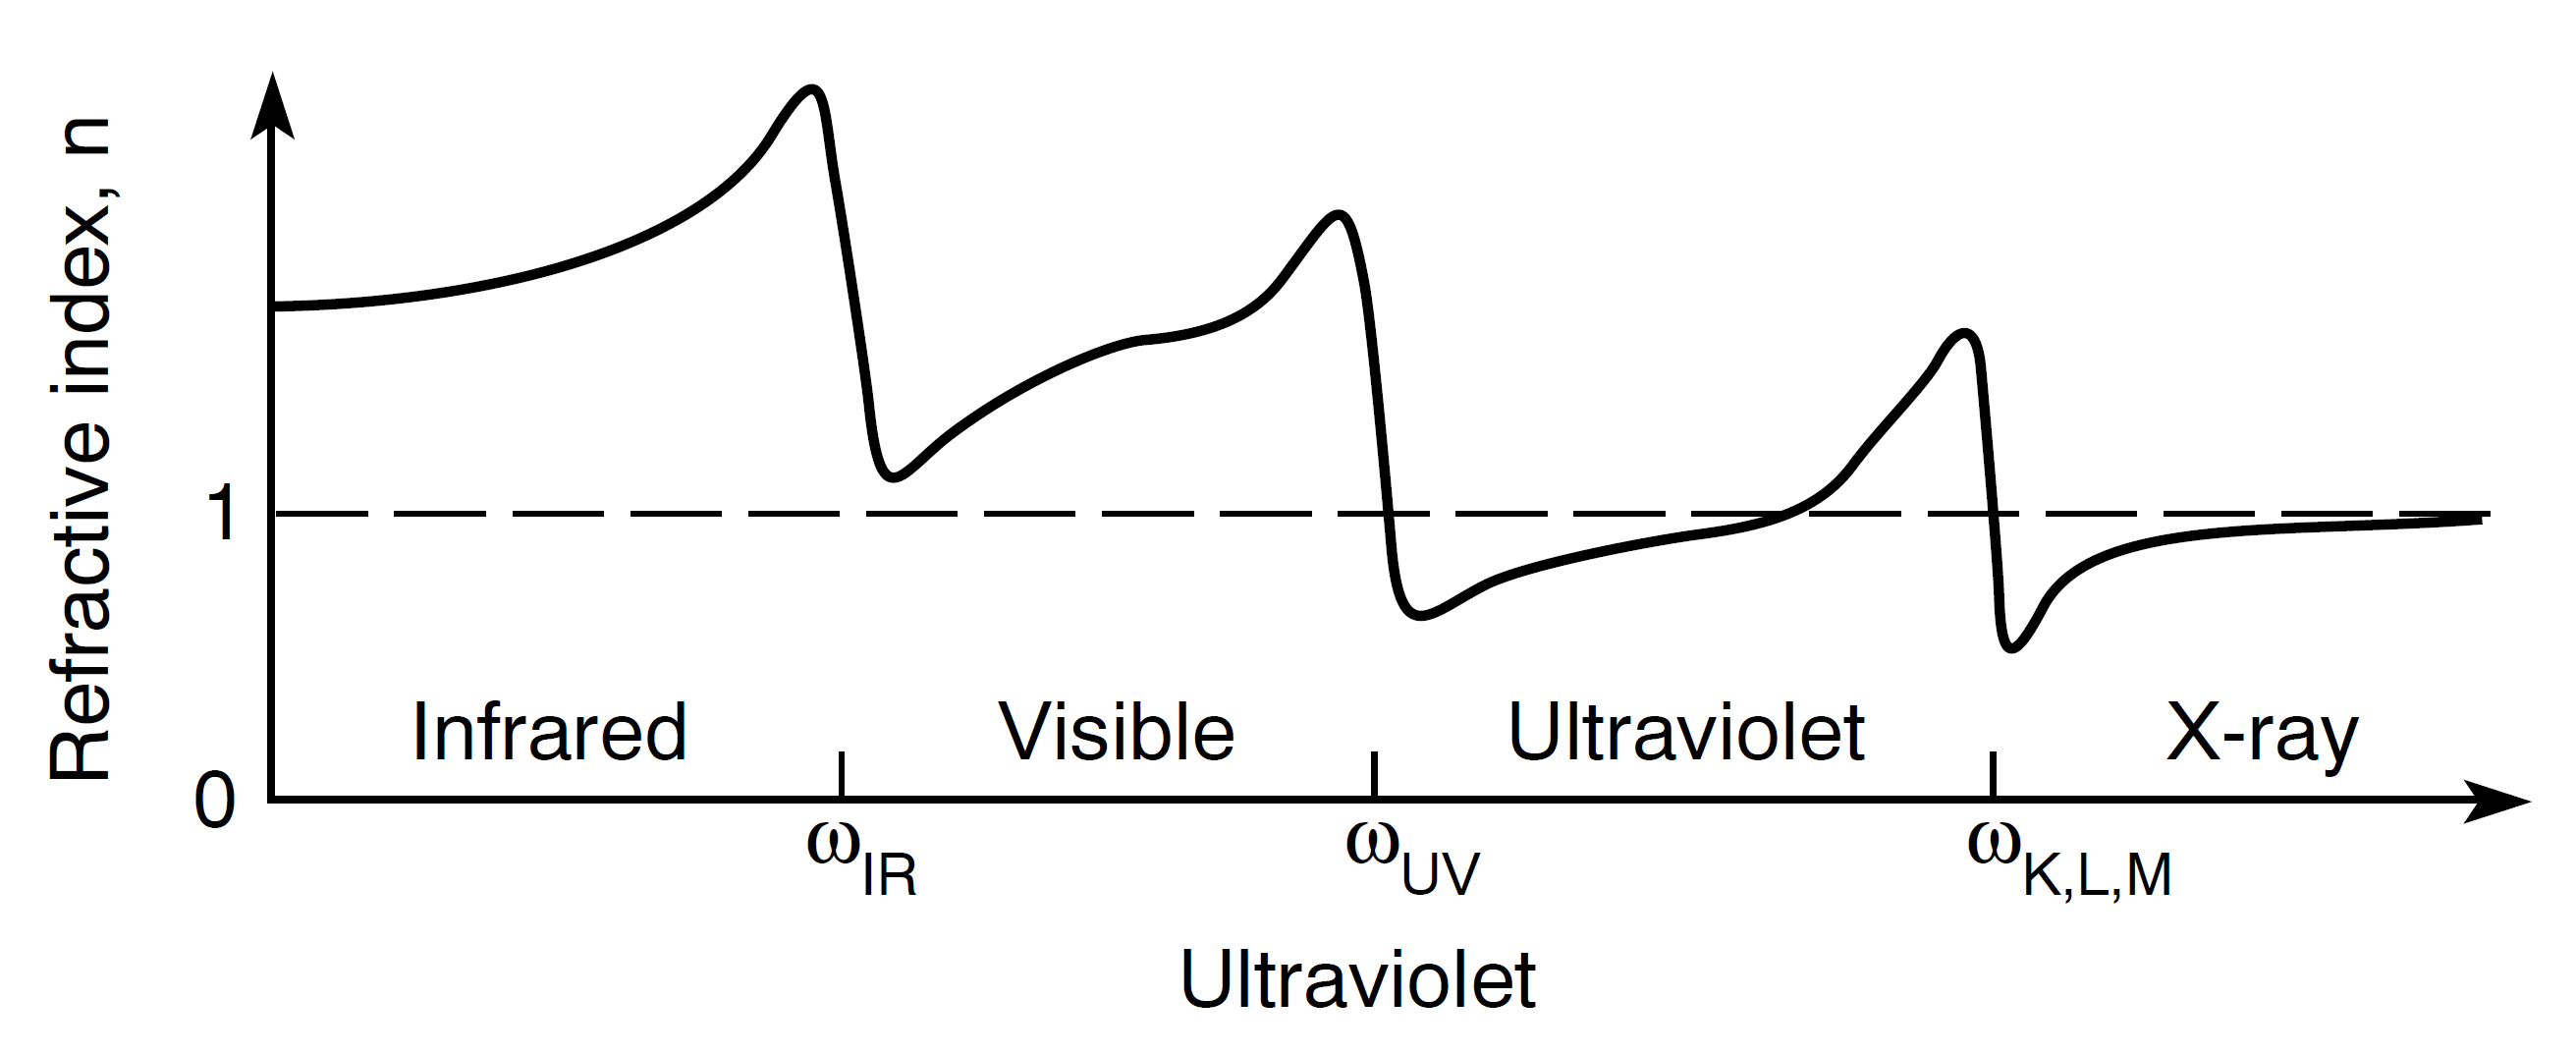
\includegraphics[width=0.7\textwidth]{figures/refractive_index/attwood_real_n_schematic.png}
	\caption{Schematic of the real part of the refractive index versus photon energy. Example resonances are shown in the IR, the visible/UV, and in the XUV/soft x-ray regimes. In general, the refractive index approaches 1 at higher photon energies.  Adapted from \cite{attwoodSoftXraysExtreme2000}.}
	\label{fig:refractive_index_schematic}
\end{figure}

In general, the complex refractive index can be written as\cite{attwoodSoftXraysExtreme2000}
\begin{equation}
\label{eqn:refractive_index}
	n(\omega)=1 - \bigg(\frac{n_a r_e \lambda^2}{2\pi}\bigg)\bigg[f_1(\omega) - i f_2(\omega)\bigg]
\end{equation}
where $n_a$ is the number density, $\omega$ ($\lambda$) is the photon energy (wavelength), and
\begin{equation}
\label{eqn:r_e}
	r_e = \frac{e^2}{4\pi\epsilon_0 mc^2}
\end{equation}
is the classical electron radius. By introducing the parameters $\beta$ and $\delta$, such that
\begin{equation}
\label{eqn:delta_beta_def}
	\begin{aligned}
	\delta &= \frac{n_a r_e \lambda^2}{2\pi}f_1(\omega)
	\beta & = \frac{n_a r_e \lambda^2}{2\pi}f_2(\omega),
	\end{aligned}
\end{equation}
then the refractive index $n$ can be written as
\begin{equation}
\label{eqn:refractive_index_db}
	n(\omega)=1-\delta+i\beta.
\end{equation}
The values of both $\delta$ and $\beta$ have been tabulated for elements from hydrogen up to uranium in the range of 10 eV to 30 keV\cite{henkeLowenergyXrayInteraction1982}, and their values are generally smaller than unity when far from resonance.

Now that we've established the form of the refractive index, we will consider the case of propagation through a dispersive medium \cite{attwoodSoftXraysExtreme2000}. The idea is to consider a plane wave of the form
\begin{equation}
	\mathbf{E}(\mathbf{r},t)=\mathbf{E}_0e^{-i(\omega t - \mathbf{k}\cdot\mathbf{r})},
\end{equation}
and assume that the dispersion of the medium takes the form
\begin{equation}
	\frac{\omega}{k}=\frac{c}{n}=\frac{c}{1-\delta+i\beta}.
\end{equation}
With these relationships, one can write the field in the propagation direction defined by $\mathbf{k}\cdot\mathbf{r}=kr$ as
\begin{equation}
\label{eqn:wave_prop}
	\mathbf{E}(\mathbf{r},t)=\big(e^{-i\omega(t - r/c)}\big) \big(e^{-i(2\pi\delta/\lambda)r}\big) \big(e^{-(2\pi\beta/\lambda)r}\big).
\end{equation}
The first term in parentheses is the wave propagation, the second term is a phase shift proportional to $\delta$ that is induced by the dispersive medium, and the third term is a decay in amplitude that is proportional to $\beta$.  From this relationship, it can be shown that the attenuation of the intensity is given by 
\begin{equation}
\label{eqn:beer-lambert}
	\frac{I}{I_0}=e^{-(4\pi\beta/\lambda)r}=e^{-n_a \sigma_a r}
\end{equation}
where $I_0$ is the initial intensity and $\sigma_a=2r_\lambda f_2(\omega)$ is the photoabsorption cross section.  This relationship shows that by measuring the absorption of a material (a thin, free-standing film for these photon energies), one can easily extract the imaginary part of the refractive index.

The effect of the real part of the refractive index is to induce a phase shift in propagating field, as can be seen from equation \ref{eqn:wave_prop}.  After propagating through a material of thickness $L$, the induced phase shift is given by
\begin{equation}
\label{eqn:phase_shift}
	\Delta\phi=\frac{2\pi\delta L}{\lambda}.
\end{equation}
To experimentally access this phase shift, the technique that can be used is interferometry \cite{hemmersDirectMeasurementComplex2012, hemmersMulticolorXUVInterferometry2009, wilsonDoubleSlitInterferometry2012}. The idea is to create a Mach-Zehnder interferometer (see figure \ref{fig:mach-zehnder_interferometer}), and in one of the arms introduce a sample of thickness $L$. By measuring how the interference patterns shift when introducing the sample, then one can directly measure the phase shift induced by the sample.  Additionally, by looking at how the fringe contrast changes, one can also get access to the attenuation caused by the sample.  This means that both the real and imaginary parts of the refractive index can be probed simultaneously.  This concept is precisely what will be used to extract the real and imaginary parts using the two XUV sources generated by a SWPG.  In that case each source will act as one arm of a Mach-Zehnder interferometer.
\begin{figure}
	\centering
	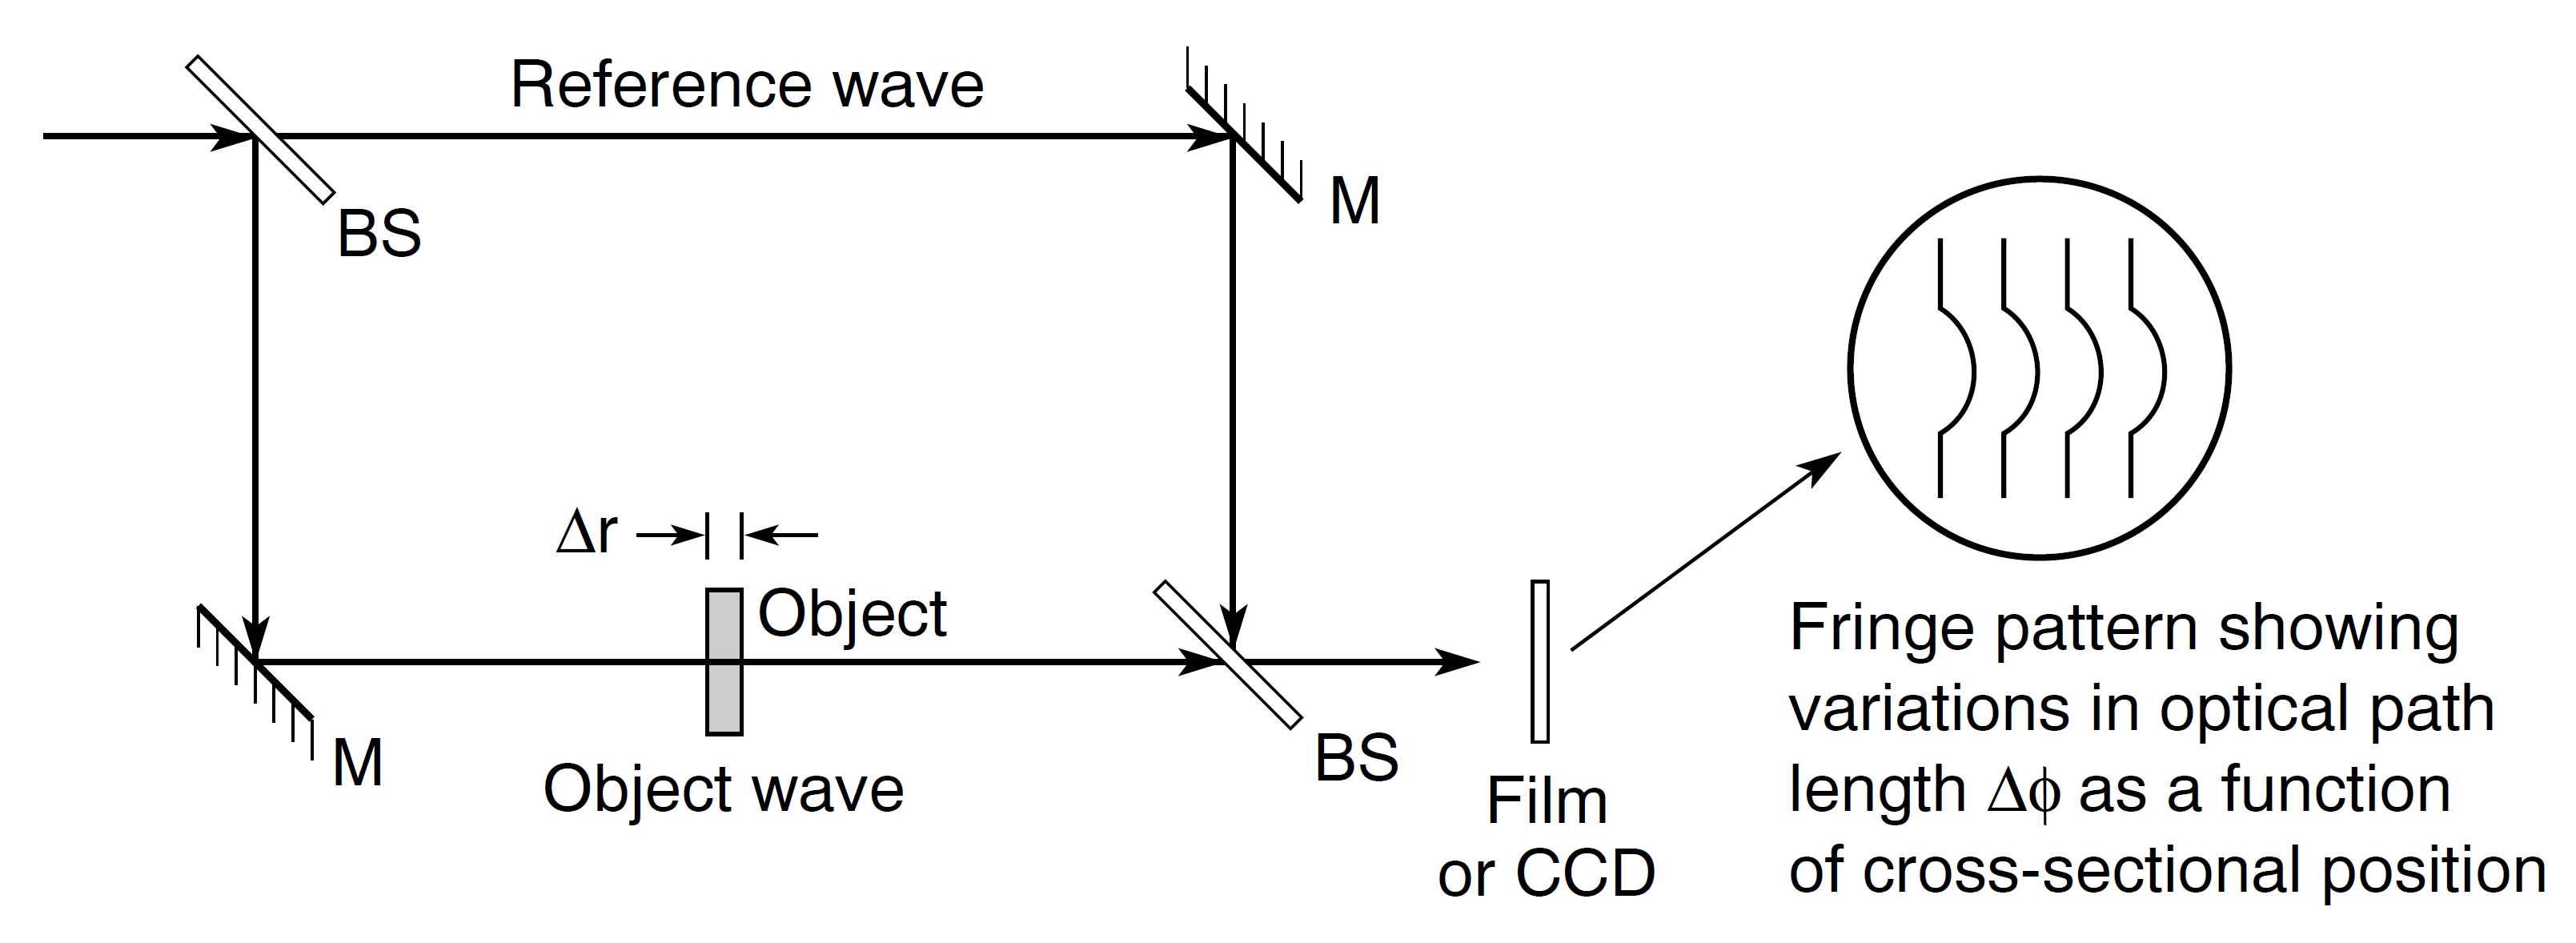
\includegraphics[width=0.7\textwidth]{figures/refractive_index/mach_zehnder_phase_shift.png}
	\caption{Schematic of a Mach-Zehnder interferometer that is used to measure the phase shift induced by a sample placed in one of the arms of the interferometer.  For the experiments described in this chapter, the two XUV sources will act as the two arms of a Mach-Zehnder.  Modified from \cite{attwoodSoftXraysExtreme2000}.}
	\label{fig:mach-zehnder_interferometer}
\end{figure}

\section{Measurement of the complex refractive index}
\subsection{Experimental setup}
\label{sec:experimental_setup_refrac}
The experimental setup that will be used to demonstrate the ability to measure both the real and imaginary parts of the refractive index is very similar to the experimental setup presented in chapter \ref{chap:two_source}.  The TABLe is the experimental beamline that will be used, and the setup is shown in figure \ref{fig:refract_schematic}.
\begin{figure}
	\centering
	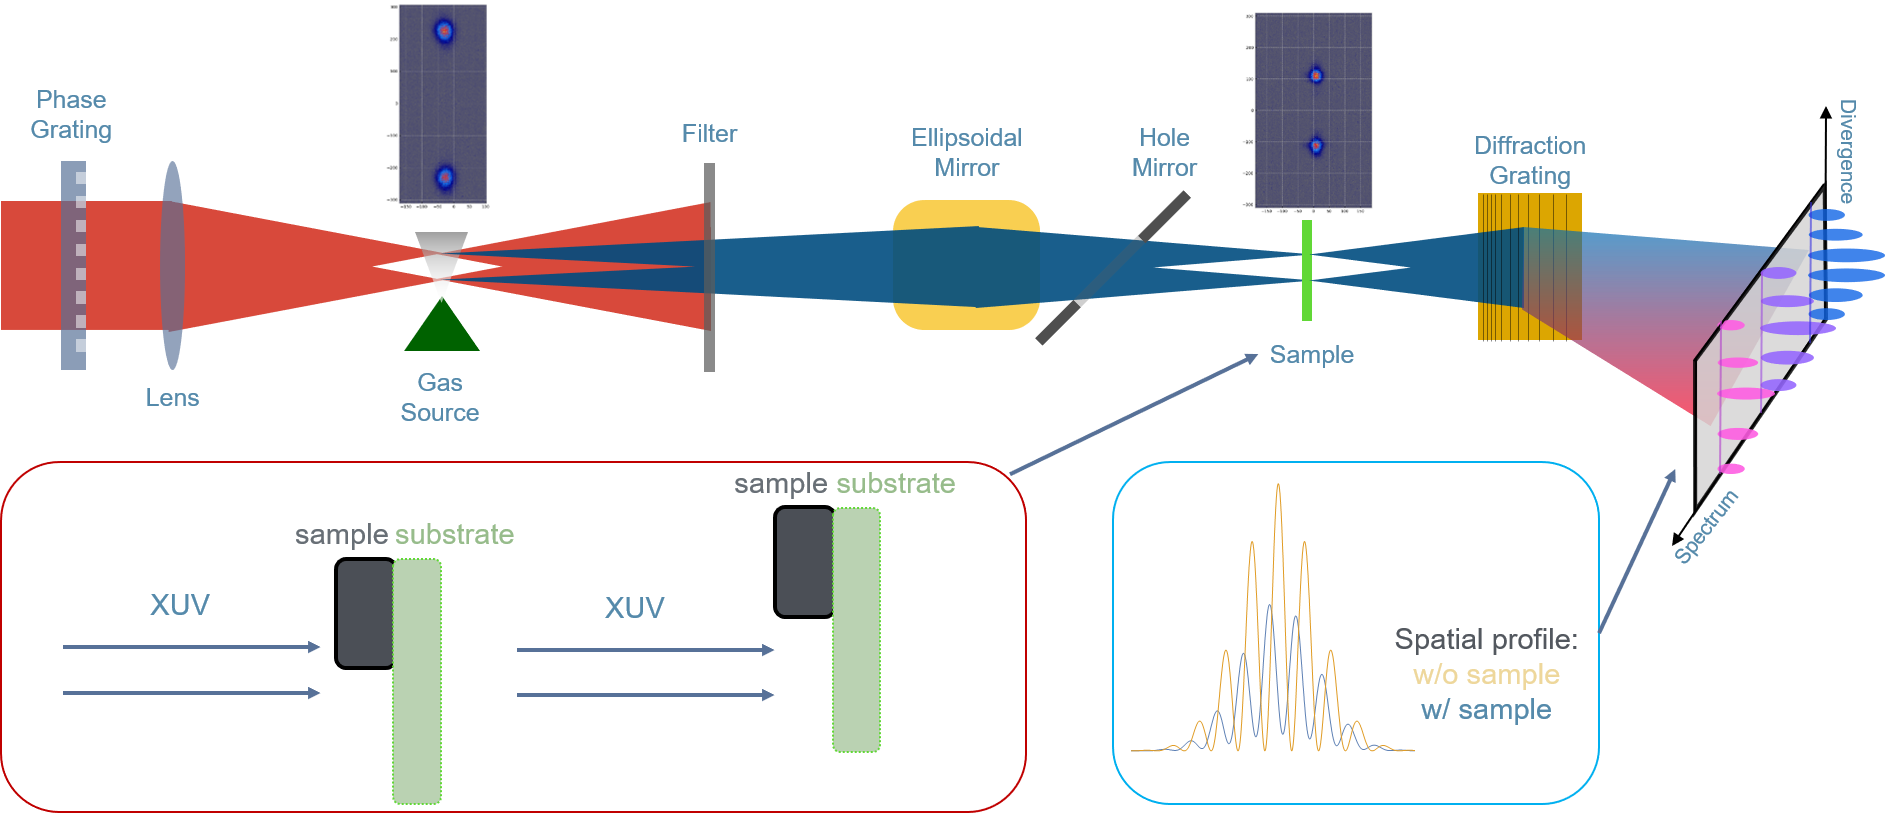
\includegraphics[width=0.8\textwidth]{figures/refractive_index/experimental_setup.png}
	\caption{Schematic of the two-source HHG experiment performed in the TABLe. A $0-\pi$ SWPG is used to generate two intense lobes at the focus of a lens.  These lobes will generate XUV beams which will interfere in the far-field.  An ellipsoidal mirror is used to refocus the XUV beams into a target chamber before going onto the spectrometer. A sample that is shaped like a step-function will be introduced at the focus of the XUV in the target chamber.  The spatial profile of the various harmonic orders will be measured in the two cases shown.  The fringe shift and fringe contrast changes allow for a simultaneous measurement of both parts of the refractive index of the sample.}
	\label{fig:refract_schematic}
\end{figure}
We use the output of the TOPAS at 1435 nm with a pulse energy of about 2 mJ and a pulse duration of around 70 fs. A $0-\pi$ SWPG is with a grating period of 2.5 mm is used to generate two intense lobes at the focal plane of a 400 mm focal length CaF2 plano-convex lens. At the focal plane, a gas medium is generated by a piezoelectric pulsed gas jet in which harmonics will be generated by the two sources.  The generation gas that will be used is argon. The fundamental wavelength is then filtered out by an aluminum filter.  The Al filter acts a high frequency bandpass with a bandpass region of 20-72 eV for the harmonic energies that are generated at this wavelength.  The harmonics are then refocused into a target chamber by an ellipsoidal mirror with a demagnification of three.  This entails that the source separation in the target chamber will be smaller by a factor of three, and the beam waist of each source will also be reduced by a factor of three.  This is where a sample will be introduced into only one of the two XUV sources.  After transmitting through the sample, the XUV will propagate to the spectrometer which allows for the spatial profile of each harmonic order to be measured.

In order to implement the scheme shown in figure \ref{fig:refract_schematic}, we need to introduce a sample into only one of the two XUV sources that are generated.  As mentioned previously, the source separation in the target chamber will be a third of the separation in the generation chamber. For the SWPG and laser parameters that we used for this experiment, the source separation in the harmonic generation chamber is $\Delta x=2\lambda f/d\approx460\:\mu m$, and the corresponding separation will be $\Delta x_t = \Delta x/3\approx153\: \mu m$ in the target chamber.  Therefore, the ideal sample has a cross sectional profile that is as close to a step function as possible, and the width of the step should be much less the separation between the two sources.  In general, this can be accomplished using photolithography techniques to pattern a thin film on top of a free standing membrane substrate.  For the sample that is used in this proof of principle experiment, we instead chose to start with a commercially available free standing membrane, and then break the membrane in such a way that it would have a sharp step-like cross sectional profile.  The membrane that was chosen was a free standing 260 nm single crystal Si membrane on a $500\:\mu m$ Si frame.  These free standing membranes are manufactured by Norcada.  The sample needs to be this thin because this experiment is done in transmission and XUV is strongly absorbed by most materials. A schematic of the sample that was used is shown in figure \ref{fig:split_sample}.
\begin{figure}
	\centering
	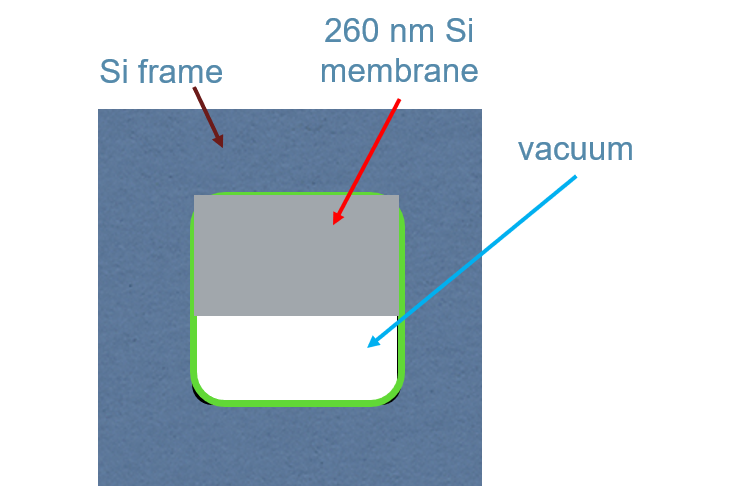
\includegraphics[width=0.5\textwidth]{figures/refractive_index/broken_sample.png}
	\caption{Schematic of the sample that was used in this experiment.  It is a free standing 260 nm Si membrane that has been broken in half.  The way that the sample was cleaved in half ensures that the edge is sharper than the separation between the two sources.  The sample was made by Norcada before it was broken.}
	\label{fig:split_sample}
\end{figure}

\subsection{Results}
To measure the complex refractive index of the silicon sample shown in figure \ref{fig:split_sample}, we will look for a fringe shift and change in fringe contrast when only one of the sources is going through the Si sample and the other is going through vacuum.  To see this, we translate the sample through the focal plane in the target chamber such that there are three distinct regimes will occur.  The first is when both samples are going through vacuum, the second is when one sample is going the sample and the other is going through vacuum, and the final regime is when both samples are going through the Si membrane.  Since this is a differential measurement, we would only expect to see a fringe shift for the second regime.  The first and third regimes should show the same fringe pattern, and the only expected difference is the overall modification of the spectral amplitude of the harmonics that due the absorption of the Si membrane.  This is shown in figure \ref{fig:harmonic_phase_shift}, where the spatial profile is shown for harmonic order 29 as the sample is translated through the focal plane.  
\begin{figure}
	\centering
	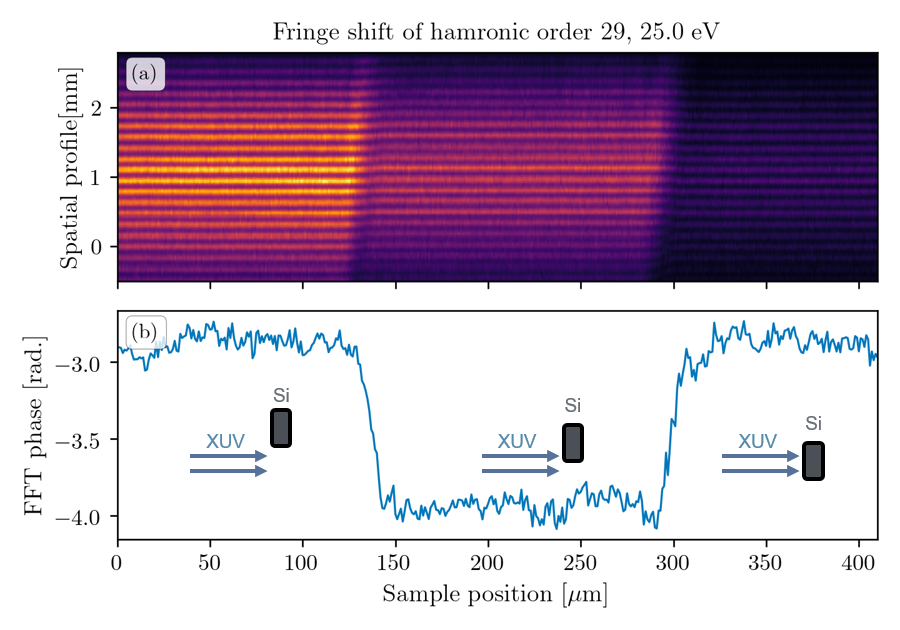
\includegraphics[width=1.0\textwidth]{figures/refractive_index/harmonic_phase_shift.png}
	\caption{(a) Spatial profile of harmonic order 29 as the silicon sample is translated through the two sources. Three regimes are clear from the spatial profile, and they correspond to both sources going through vacuum, only one source going through the sample, and both sources going through the sample.  A clear fringe shift can be seen between the second regime and the other two.  Additional structure is seen at the transition between regimes, and this is due to diffraction cause by the sample partially blocking one of the sources. (b) Phase extracted from the spatial frequency corresponding to this harmonic order.  The phase shift induced by the Si sample can be extracted from this phase shift.}
	\label{fig:harmonic_phase_shift}
\end{figure}
From the spatial profile shown in figure \ref{fig:harmonic_phase_shift}, the three expected regimes can clearly be seen.  There is also additional spatial structure that is present in the transition between each of the three regimes.  This is due to diffraction that is caused by one of the sources being partially blocked.  From the spatial profile, the fringe shift can be extracted from the spatial frequency component that corresponds to this harmonic.  The phase of that spatial frequency is plotted in \ref{fig:harmonic_phase_shift} and shows that there is a phase shift between the two sources when only one of the sources is going the sample.  From this phase shift it is now possible to calculate the real part of the refractive index from the relationship $\Delta \phi = 2\pi\delta L/\lambda$ where $\Delta \phi$ is the phase shift between the two sources.  The phase shift that is observed in harmonic order 29 can be seen across the harmonic spectrum, and enables the real part of the refractive index to be extracted across a broad range of photon energies simultaneously.

\begin{figure}
	\centering
	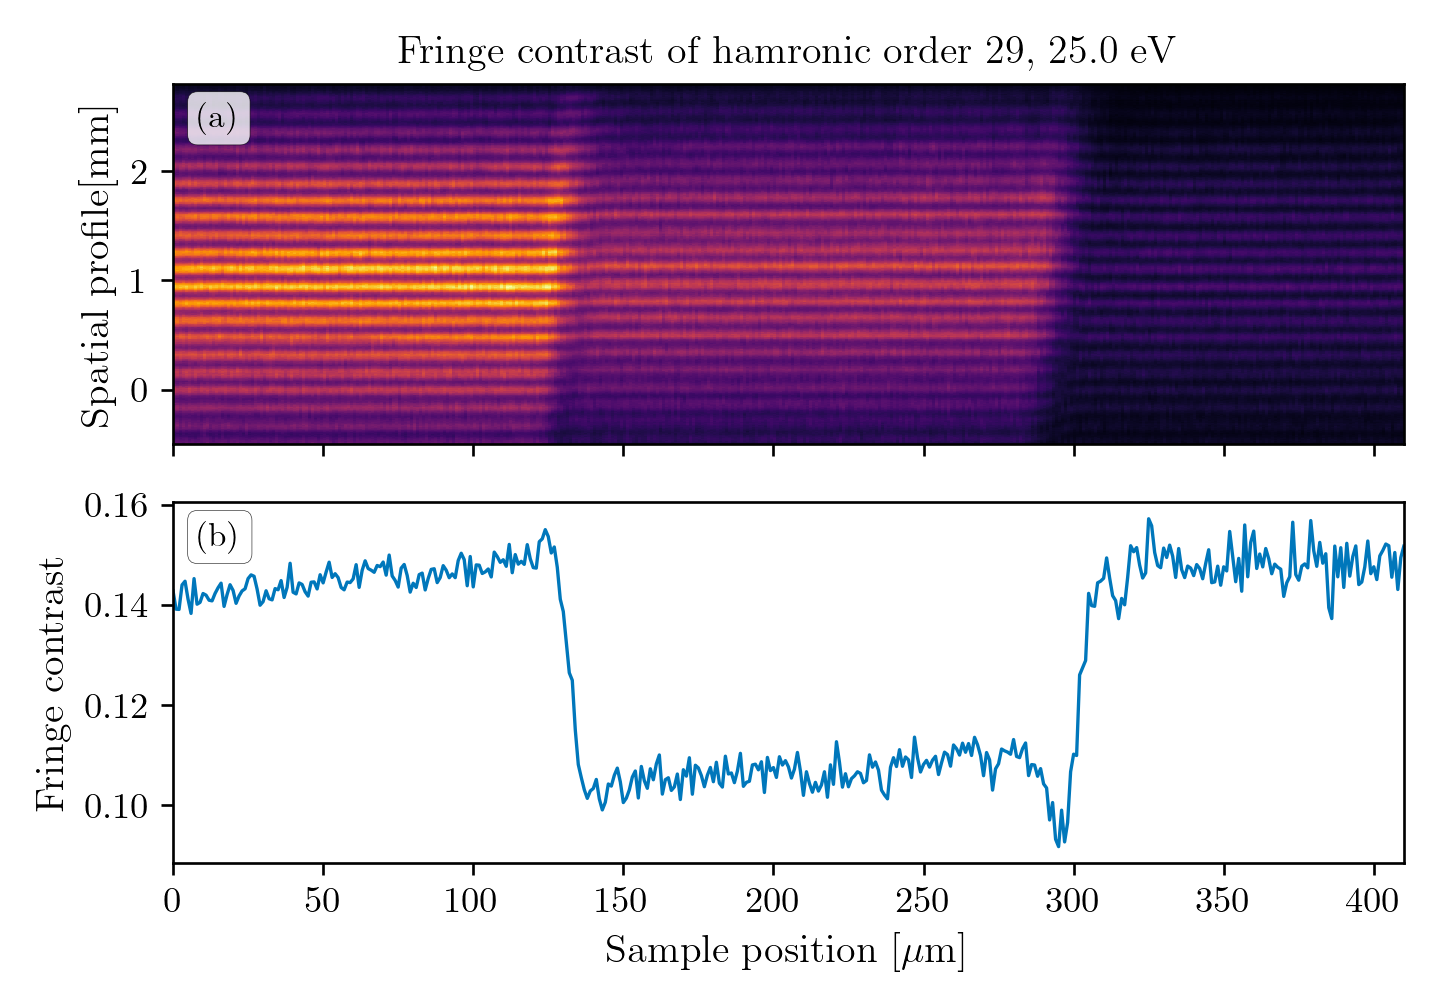
\includegraphics[width=1.0\textwidth]{figures/refractive_index/spatialgram_fringe_contrast.png}
	\caption{(a) Spatial profile of harmonic order 29 as the silicon sample is translated through the two sources. Three regimes are clear from the spatial profile, and they correspond to both sources going through vacuum, only one source going through the sample, and both sources going through the sample. (b) Fringe contrast extracted from the spatial frequency corresponding to this harmonic order.}
	\label{fig:harmonic_fringe_contrast}
\end{figure}
In addition to the fringe shift that is show in figure \ref{fig:harmonic_phase_shift}, there is also a change in fringe contrast that can be seen as the sample is translated through the two sources.  This change in fringe contrast is shown in figure \ref{fig:harmonic_fringe_contrast}.  The contrast shows the three distinct regimes that were seen in the fringe shift.  Similarly to the fringe shift, it can be seen that there is only a change in fringe contrast when only one of the sources is going through the sample.  From this contrast, it is possible to calculate the imaginary part of the refractive index. 

\begin{figure}
	\centering
	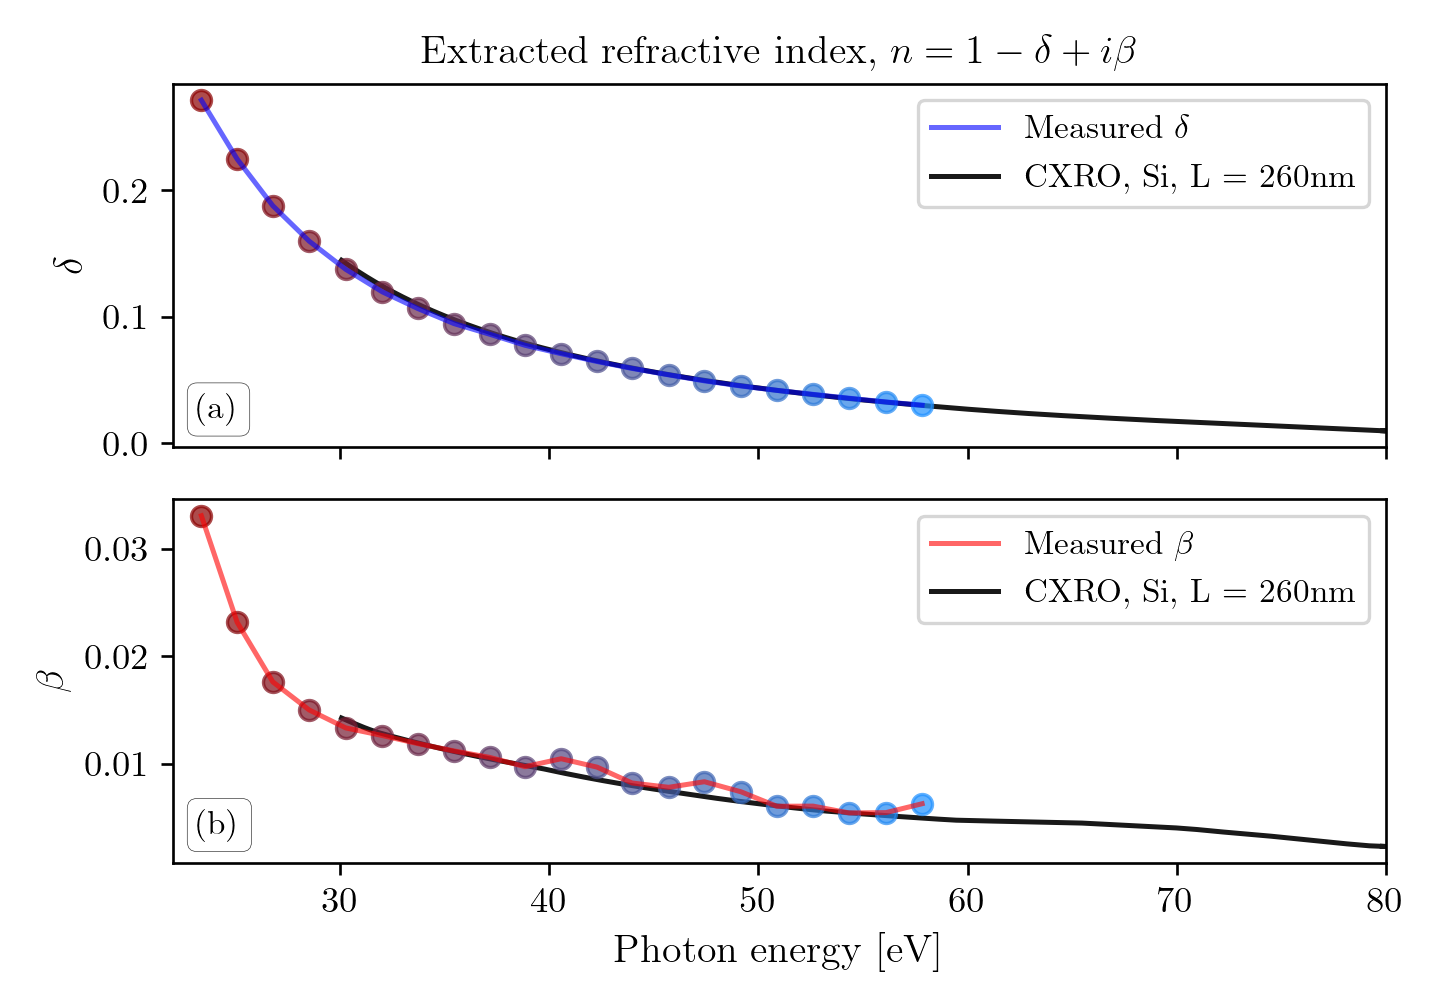
\includegraphics[width=1.0\textwidth]{figures/refractive_index/db_cxro.png}
	\caption{(a) Real part of the refractive index measured using a SWPG.  Shows excellent agreement with the values from CXRO. (b) Imaginary part of the refractive index measured using a SWPG.  Overall shape agrees with CXRO, however there is a factor of 2 difference in amplitude.}
	\label{fig:measured_delta_beta}
\end{figure}
By combining both the fringe shift and the change in fringe contrast, we can now calculate both the real and imaginary part of the refractive index of Si over the range 25 - 60 eV.  The results are shown in figure \ref{fig:measured_delta_beta}.  As can be seen in the figure, there is excellent agreement between the measured real part when compared to the values that can be obtained from CXRO \cite{henkeXRayInteractionsPhotoabsorption1993}.  The imaginary part shows a factor of 2 difference in amplitude, however the overall shape agrees well with CXRO. The origin of the amplitude difference is still being analyzed.

\section{Conclusion}
In this chapter, the complex refractive index was introduced and a method to measure both the real and imaginary parts was proposed. The method relies on the use of a $0-\pi$ SWPG to generate two relative phase locked XUV sources whose interference acts as an inline Mach-Zehnder interferometer.  By introducing a sample into one of the sources, the corresponding fringe shift and change in fringe contrast gives access to the real and imaginary parts of the refractive index.  A sample of Si was fabricated to test this method, and measuring it's refractive index shows excellent agreement between our measured results and the literature. By demonstrating that it is possible to accurately extract both the real and imaginary parts, we have accurately characterized the ground state of a condensed matter system.  The next step is to extract the dynamic real and imaginary parts that are induced by dressing the sample with another IR field.  This will be discussed in a later chapter.



